\documentclass[aspectratio=169,compress,x11names]{beamer}
\usefonttheme[onlymath]{serif}
\setbeameroption{hide notes} % Only slides
\usetheme{Boadilla}
	\setbeamertemplate{navigation symbols}{}
	\setbeamertemplate{headline}{%
	\leavevmode%
	\hbox{%
		\begin{beamercolorbox}[wd=\paperwidth,ht=2.5ex,dp=1.125ex]{section in head/foot}%
			\insertsectionnavigationhorizontal{\paperwidth}{}{\hskip0pt plus1filll}
		\end{beamercolorbox}%
	}%
	\vspace*{-1em}  % Giảm khoảng trống phía dưới thanh điều hướng
}
\usepackage{tikz-feynman}
\usepackage{array}
\usepackage{animate}
\usepackage{amsmath}

\usepackage{cancel}
\usepackage{multicol}
\usepackage{physics}
\usepackage{xcolor}
\usepackage{graphicx,subcaption}
\usepackage{amssymb}
\usepackage{hyperref}
%\hypersetup{colorlinks = true,linkcolor = black,filecolor= black,urlcolor= black}
\usepackage{cancel}
\usepackage{subcaption}
\usepackage{comment}

\usepackage[backend=bibtex,bibencoding=utf8,doi=false,isbn=false,url=false,eprint=false,indexing=false,style=reading]{biblatex}
\addbibresource{refs.bib}
\AtEveryBibitem{%
	\clearname{translator}%
	\clearlist{publisher}%
	\clearfield{pagetotal}%
}
\setbeamertemplate{bibliography item}{}


\newcommand{\biblion}[3]{
	\bibitem{}  
	#1, {\color{black}\textit{#2}}, {\color{LightSteelBlue3}#3} \\
}



\makeatletter
\renewcommand\@makefnmark{\hbox{\@textsuperscript{\usebeamercolor[fg]{footnote mark}\usebeamerfont*{footnote mark}[\@thefnmark]}}}
\renewcommand\@makefntext[1]{{\usebeamercolor[fg]{footnote mark}\usebeamerfont*{footnote mark}[\@thefnmark]}\usebeamerfont*{footnote} #1}
\makeatother

\usepackage{xparse}

\usepackage[toc,page]{appendix}
\author{Tran Khoi Nguyen}
% Title page details: 
\author[Presenter: Tran Khoi Nguyen]{{\textit{Presenter}} \\
	Tran Khoi Nguyen \inst{1} \\
	{\and} \\
	{\textit{Supervisors}} \\
	Dr. Huynh Thanh Duc \inst{2}}
\institute[HCMUS]{\inst{1} University of Science, Ho Chi Minh city\and %
	\inst{2} Institute of Applied Mechanics and Informatics}
% Title page details: 
\title[Hofstadter butterfly of TMD]{Hofstadter butterfly in transistion metal dichalcogenide monolayers}
	
\date{Jul, 2025}
\logo{\includegraphics[height=0.9cm]{pic/logo1.png}\vspace*{-.055\paperheight}\hspace*{.85\paperwidth}}


\begin{document}
	\setbeamertemplate{logo}{}
	\begin{frame}
		\titlepage
	\end{frame}
	\logo{}
	\begin{frame}{Table of Contents}
		\tableofcontents
		\note{note text}
	\end{frame}
	\section{Overview}
	\begin{frame}{Overview}
		Group VI-B Transition Metal Dichalcogenides (TMD) are compound semiconductors of the type $MX_2$
		\begin{figure}
			\centering
			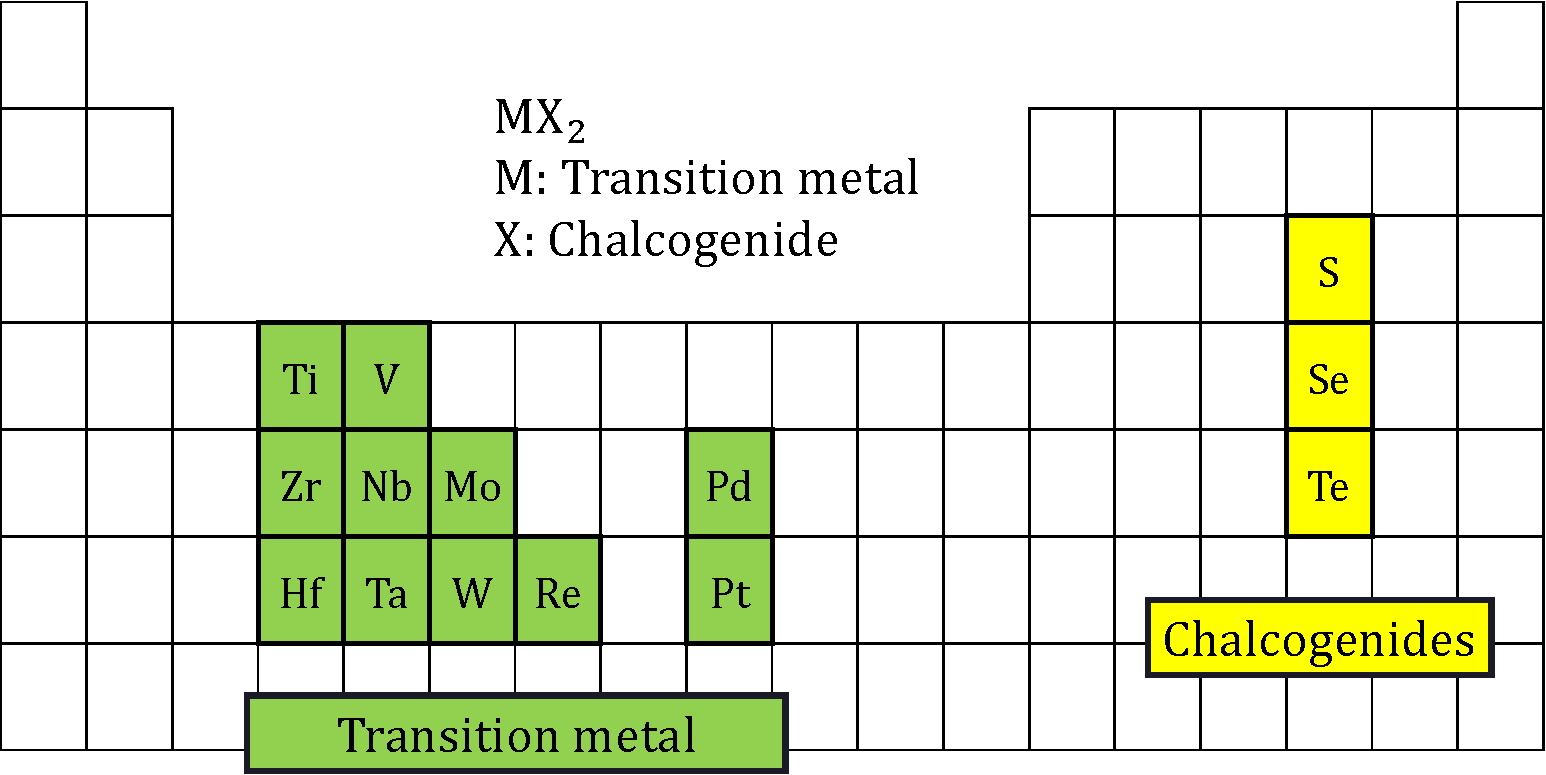
\includegraphics[width=0.65\linewidth]{./pic/periodictable.pdf}
			\caption{Transition metal dichalcogenides compound.}
		\end{figure}
	\end{frame}
	\begin{frame}{Transition Metal Dichalcogenides Monolayers}
		\begin{multicols}{2}
			\begin{itemize}
				\item One $\color{green}M$ layer sandwiched by two $\color{yellow}X$ layers as show in top view (a) and side view (b).
				\item Crystal structure has no central inversion symmetry.
				\item The symmetry of the lattice results in the hexagon Brillouin Zone (BZ).
			\end{itemize}
			\columnbreak
			\vfil
			\begin{figure}
				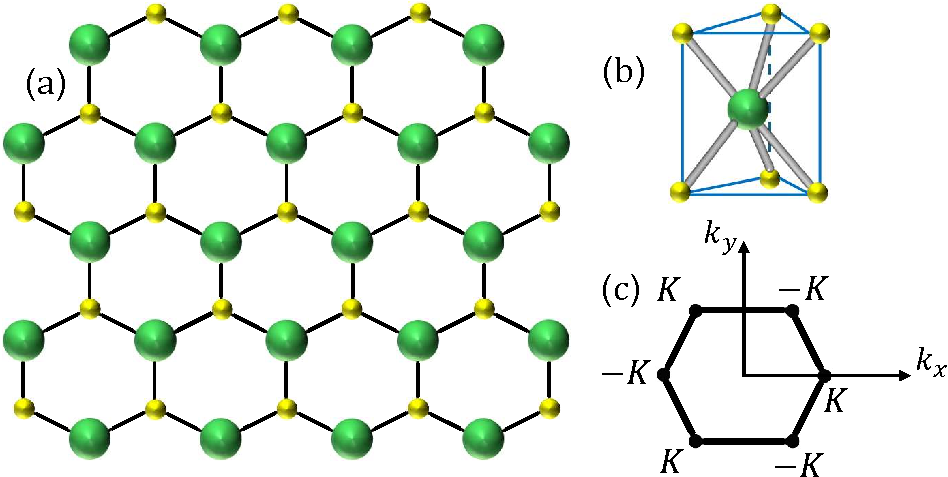
\includegraphics[width=\linewidth]{./pic/latticePresent.pdf}
				\caption{Structure and Brillouin Zone of Monolayer TMD, redrawing from \footcite{liu_three-band_2013}.}
			\end{figure}
		\end{multicols}
	\end{frame}
	\begin{frame}{Transition Metal Dichalcogenides Monolayers}
		\begin{block}{Properties}
			\begin{itemize}
				\item Both mono-layer and few-layers remain stable at room temperature.
				\item TMD monolayer has the visible band gap in the ban structure, which can be used in creating the transistor devices\footnotemark.
				\item  Strong spin-orbit coupling (SOC) in TMD monolayers lead to spin splitting of hundres meV.
			\end{itemize}
		\end{block}
		$\Rightarrow$ Promising material in electronic and optoelectronic applications.
		\footnotetext{\cite{radisavljevic2011}}
	\end{frame}
	\section{Method}
	\subsection{Three-band tigh-binding model without magnetic field}
	\begin{frame}{Three-band tigh-binding model without magnetic field}
		Time-independent Schr\"{o}dinger equation for an electron in the crystal
		\begin{gather}
			\left[-\frac{\hbar^{2} \boldsymbol{\nabla}^{2}}{2m} + U_{0}(\mathbf{r})\right] \ket{\psi_{\lambda,\mathbf{k}}(\mathbf{r})} = \epsilon_{\lambda,\mathbf{k}} \ket{\psi_{\lambda,\mathbf{k}}(\mathbf{r})}.
		\end{gather}
		Tight-binding (TB) wave function
		\begin{gather}
			\ket{\psi_{\lambda,\mathbf{k}}(\mathbf{r})} = \sum_{j} C_{j}^{\lambda}(\mathbf{k}) \sum_{\mathbf{R}} e^{i \mathbf{k} \cdot \mathbf{R}} \ket{\phi_{j} (\mathbf{r} - \mathbf{R})}.
		\end{gather}
		The basis consists of three $d$-orbitals of the $M$ atom:
		\begin{gather}
			\ket{\phi_{1}} = \ket{d_{z^{2}}} , 
			\ket{\phi_{2}} = \ket{d_{xy}} , 
			\ket{\phi_{3}} = \ket{d_{x^{2} - y^{2}}}.
		\end{gather}
		The coefficents $C_{j}^{\lambda}(\mathbf{k})$ are the solutions of the eigenvalue equation
		\begin{gather}
			\sum_{jj'}^{3} \left[H_{jj'}^{\text{TB}}(\mathbf{k}) - \varepsilon_{\lambda}(\mathbf{k}) S_{jj'}(\mathbf{k})\right] C_{j}^{\lambda}(\mathbf{k}) = 0.
		\end{gather}
	\end{frame}
	\begin{frame}{Three-band tigh-binding model without magnetic field}
		Overlap matrix elements
		\begin{gather}
			S_{jj'}(\mathbf{k}) = \sum_{\mathbf{R}} \bra{\phi_{j}(\mathbf{r})} \ket{\phi_{j'}(\mathbf{r - R})} \approx \delta_{jj'}.
		\end{gather}
		TB Hamiltonian matrix elements
		\begin{gather}
			H_{jj'}^{\text{TB}}(\mathbf{k}) = \sum_{\mathbf{R}} e^{i \mathbf{k \cdot R}} \bra{\phi_{j}(\mathbf{r})} \left[-\frac{\hbar^{2} \nabla^{2}}{2m} + U_{0}(\mathbf{r})\right] \ket{\phi_{j'}(\mathbf{r - R})}.
		\end{gather}
	\end{frame}
	\begin{frame}{Three-band tigh-binding model without magnetic field}
		\begin{figure}
			\centering
			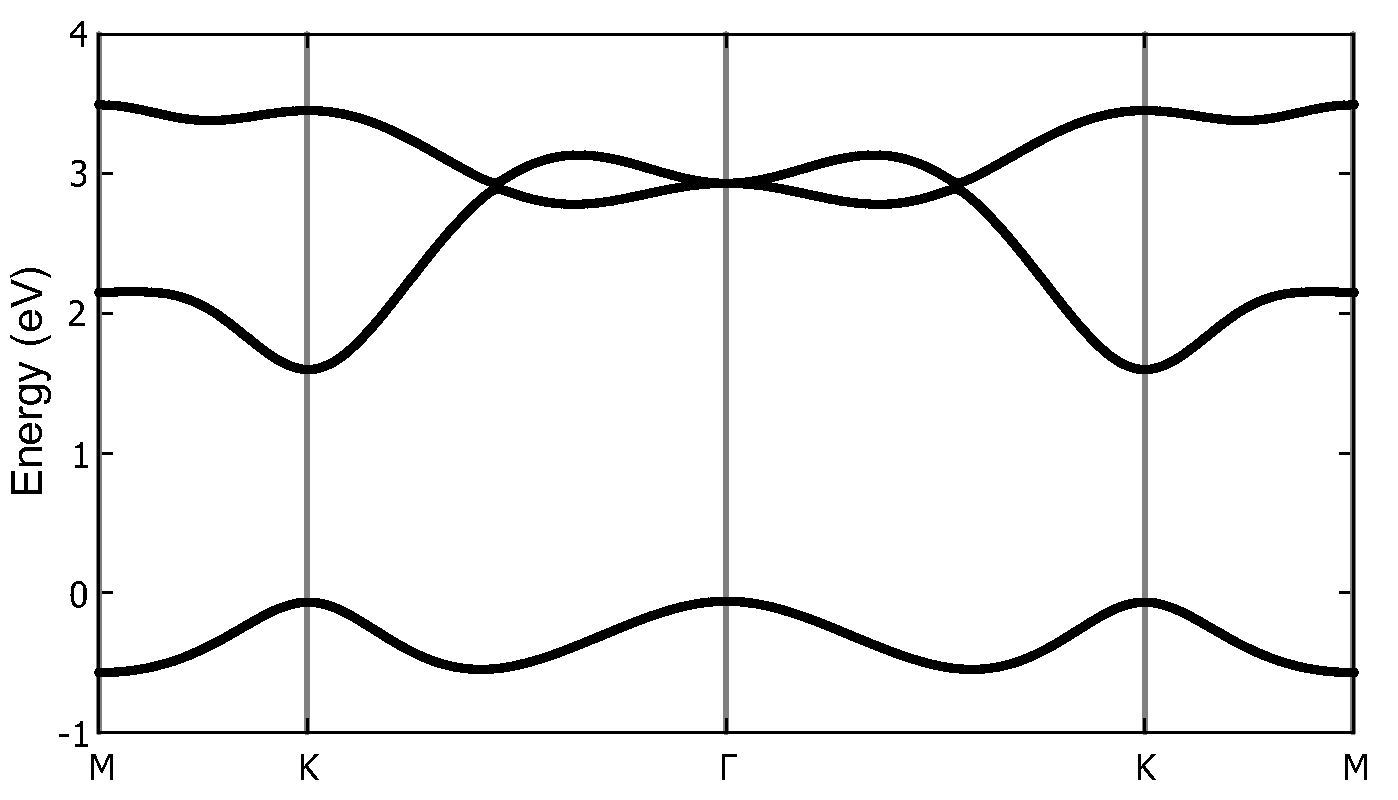
\includegraphics[width=0.65\linewidth]{./pic/bandstructure.pdf}
			\caption{Band structure of $MoS_{2}$ monolayer\footcite{liu_three-band_2013}.}
		\end{figure}
	\end{frame}

	\subsection{Three-band tigh-binding model under a magnetic field}
	\begin{frame}{Three-band tigh-binding model under a magnetic field}
		TB Hamiltonian matrix elements change to
		\begin{gather}
			H= \frac{(-i \hbar \boldsymbol{\nabla} + e \mathbf{A}(\mathbf{r}))^{2}}{2m} + U_{0}(\mathbf{r}) + g^{*} \mu_{B} \mathbf{B} \cdot \mathbf{L},
		\end{gather}
		It is possible to add a phase factor to the basis functions
		\begin{gather}
			\psi_{\lambda,\mathbf{k}}(\mathbf{r}) = \sum_{j=1}^{3} C_{j}^{\lambda}(\mathbf{k}) \sum_{\mathbf{R}} e^{i (\mathbf{k} \cdot \mathbf{R} + \theta_\mathbf{R}(\mathbf{r}))} \phi_{j}(\mathbf{r} - \mathbf{R}).
		\end{gather}
		By choosing $\theta_\mathbf{R} = - \tfrac{e}{\hbar} \int_{\mathbf{R}}^{\mathbf{r}} \mathbf{A}(\mathbf{r'}) \cdot d\mathbf{r}' $ as Peierls substitution, the Hamiltonian matrix elements as the form
		\begin{equation}
			\begin{aligned}
				H_{jj'}^{\text{TB}}(\mathbf{k})
				&= \sum_{\mathbf{R}} e^{i\mathbf{k \cdot R} + \frac{ie}{\hbar} \int_{\mathbf{0}}^{\mathbf{R}} \mathbf{A(\mathbf{r'})} \cdot d \mathbf{r'} } \bra{\phi_{j}(\mathbf{r})} \left[ -\frac{\hbar^{2} \boldsymbol{\nabla}^{2}}{2m} + U_{0} (\mathbf{r}) \right] \ket{\phi_{j'}(\mathbf{r - R})} \\
				&+ g^{*} \mu_{B} \mathbf{B} \cdot \sum_{\mathbf{R}} e^{i\mathbf{k \cdot R} + \frac{ie}{\hbar} \int_{\mathbf{0}}^{\mathbf{R}} \mathbf{A(\mathbf{r'})} \cdot d\mathbf{r'} } \bra{\phi_{j}(\mathbf{r})} \mathbf{L} \ket{\phi_{j'}(\mathbf{r - R})}.
			\end{aligned}
		\end{equation}
	\end{frame}
	\begin{frame}
		\begin{figure}
			\centering
			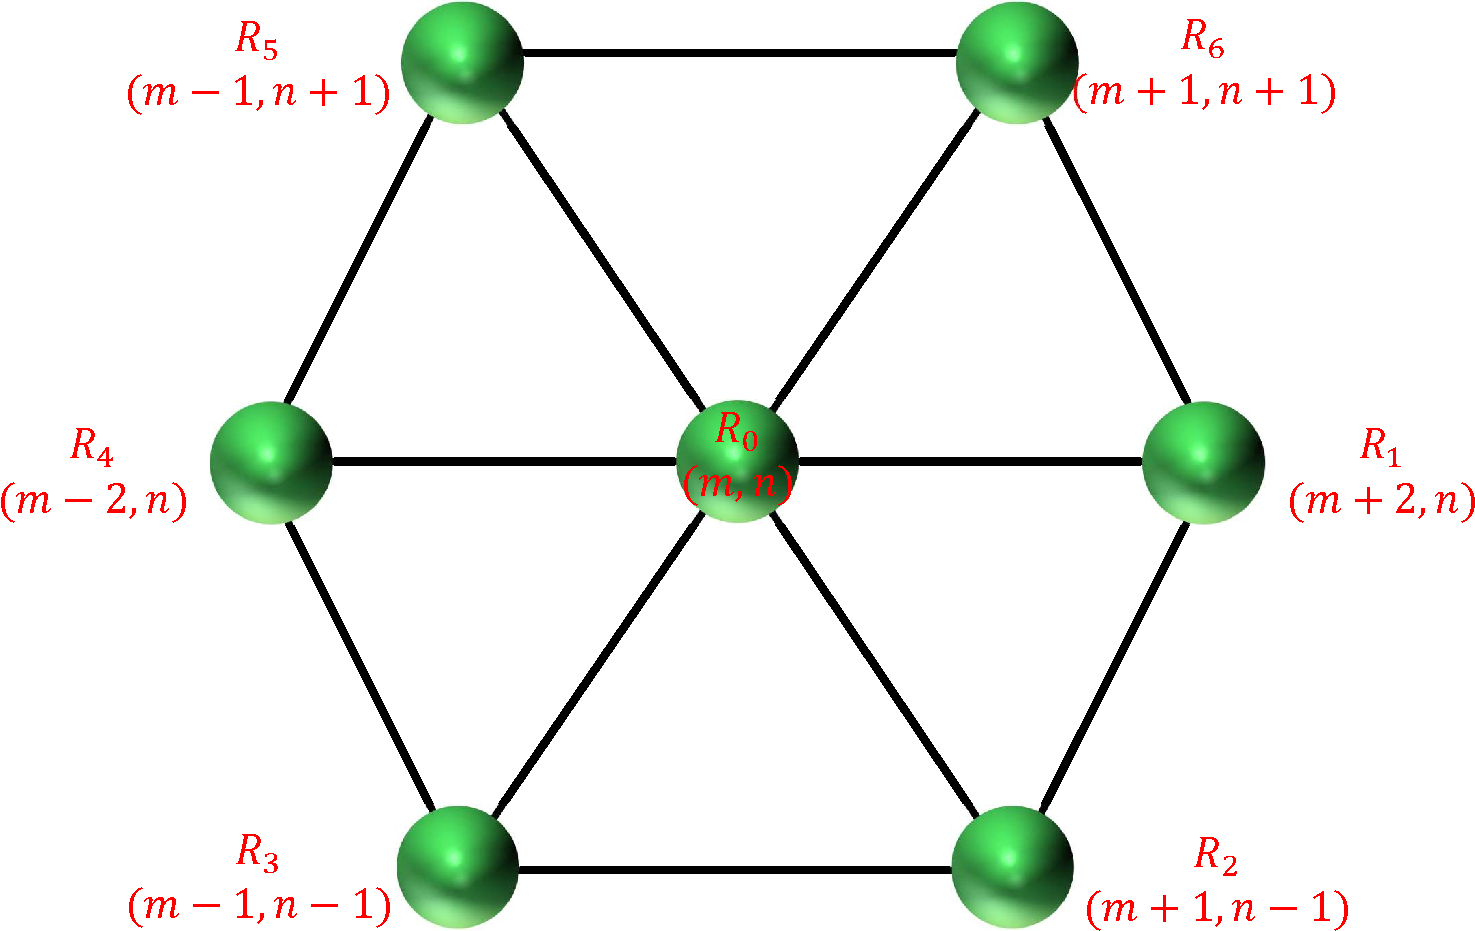
\includegraphics[width=0.5\linewidth]{./pic/siteindex_crop.pdf}
			\caption{\label{fig:site index} The TB model of TMDC with six neighbors atom $M$.}
		\end{figure}
	\end{frame}
	\begin{frame}{Three-band tigh-binding model under a magnetic field}
		\begin{figure}
			\centering
			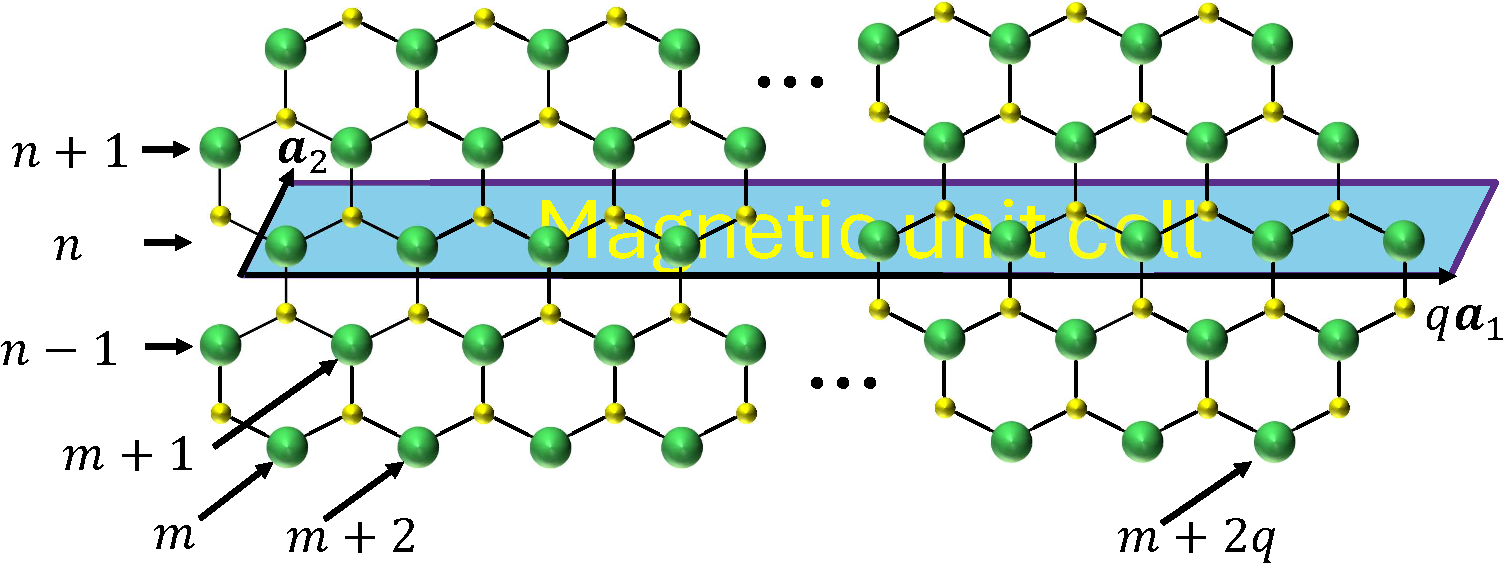
\includegraphics[width=0.85\textwidth,height=0.35\linewidth]{pic/magneticUC_cut.pdf}
			\caption{\label{fig:Mag UC} Magnetic unit cell for TMD monolayers.}
		\end{figure}
	\end{frame}
	\begin{frame}{Three-band tigh-binding model under a magnetic field}
		\begin{figure}
			\centering
			\begin{subfigure}[b]{0.495\textwidth}
				\centering
				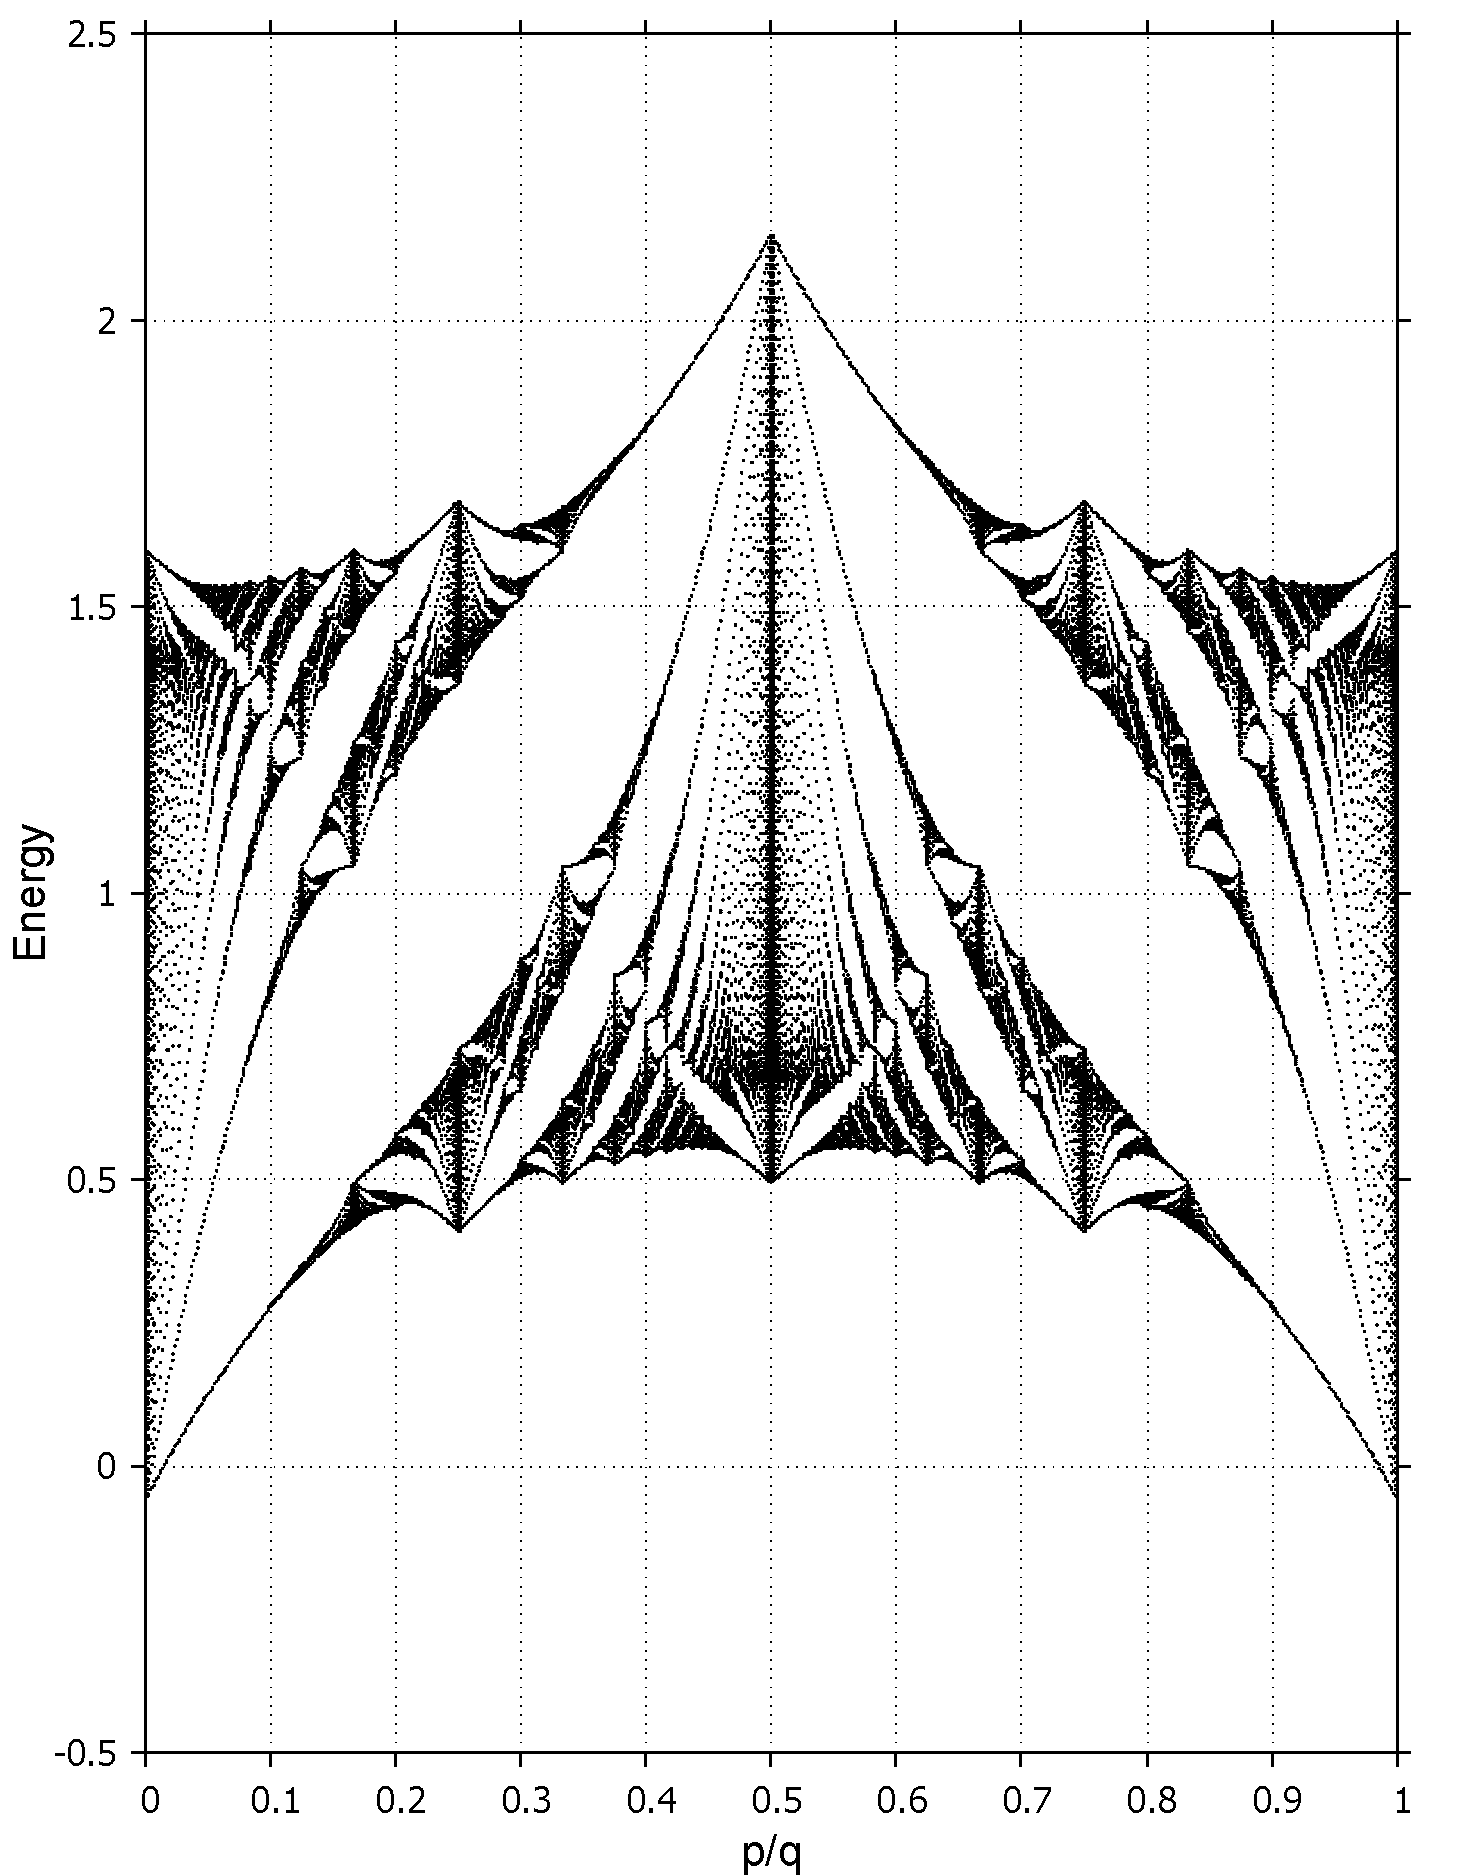
\includegraphics[width=0.65\linewidth]{../pic/h0_tam giac_q_797.png}
				\label{fig:3 band}
			\end{subfigure}
			\begin{subfigure}[b]{0.495\textwidth}
				\centering
				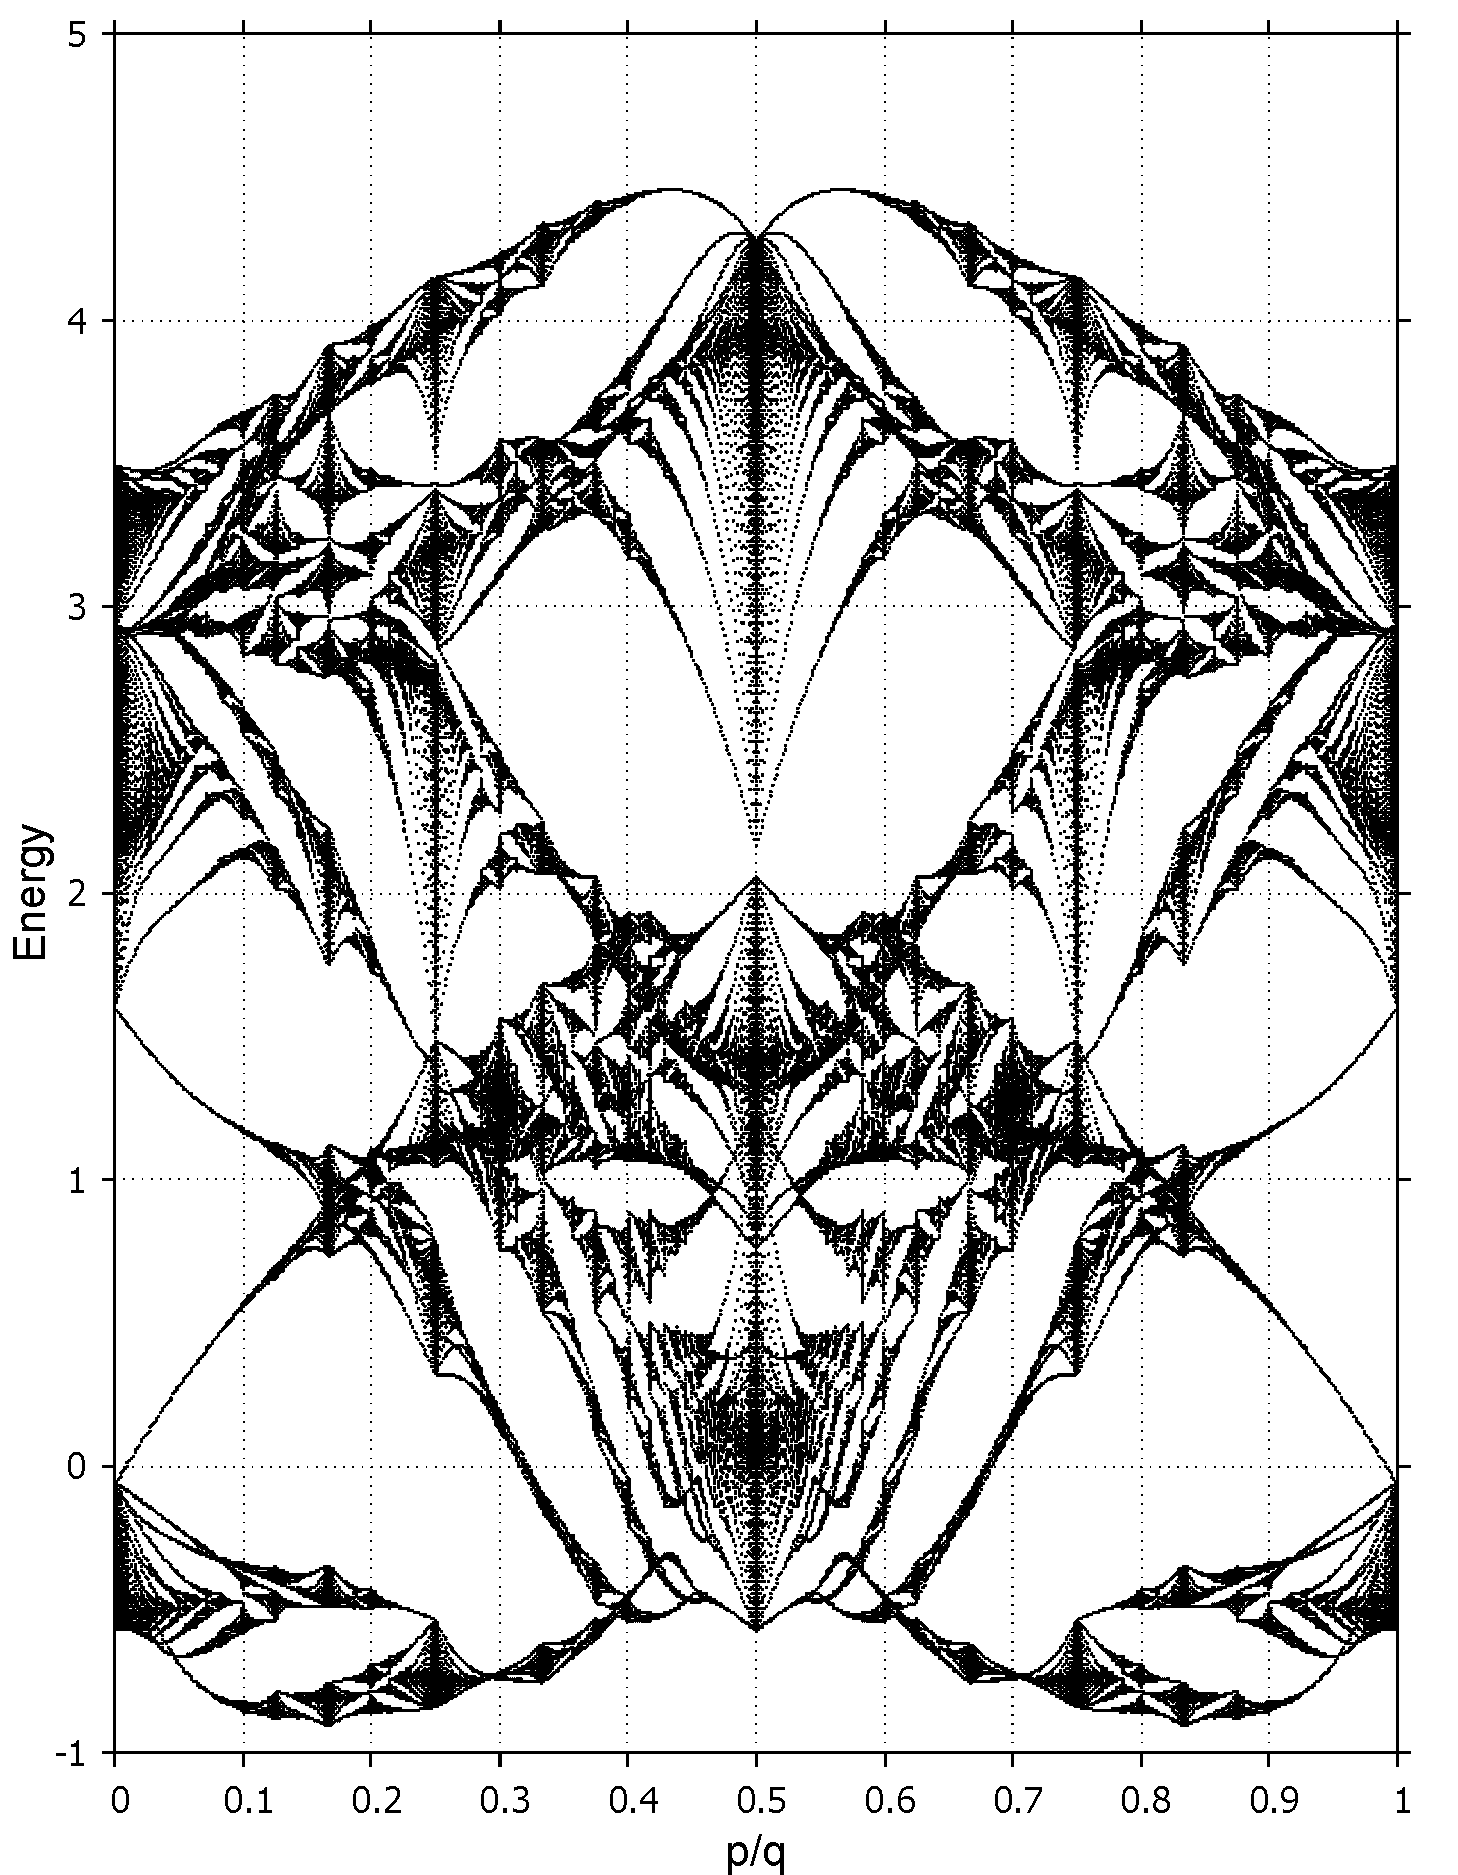
\includegraphics[width=0.65\linewidth]{../pic/3band_gnuplot_q_797.png}
				\label{fig:1 band}
			\end{subfigure}
			\caption{
				Hofstadter butterfly for single-band $\ket{dz} \equiv \ket{\phi_{1}^{1}(x,y)}$(left) and three-band(right) with $q = 797$ with field strength $B_{0} = 4.6928 \times 10^{4}$ T.
			}
		\end{figure}
	\end{frame}
 \begin{frame}
		\frametitle{Hofstadter butterfly}
		\begin{multicols}{2}
			\begin{minipage}{\columnwidth}
				\begin{block}{Properties}
					\begin{itemize}
						\item 
						\item 
						\item The spectrum also invariant under reversal of the magnetic field $\tfrac{p}{q} \to -\tfrac{p}{q}$.
						\item At weak magnetic field, Landau levels can clearly seen from the Hofstadter spectrum.
					\end{itemize}
				\end{block}
			\end{minipage}
			\begin{minipage}{\columnwidth}
				\begin{figure}
					\centering
					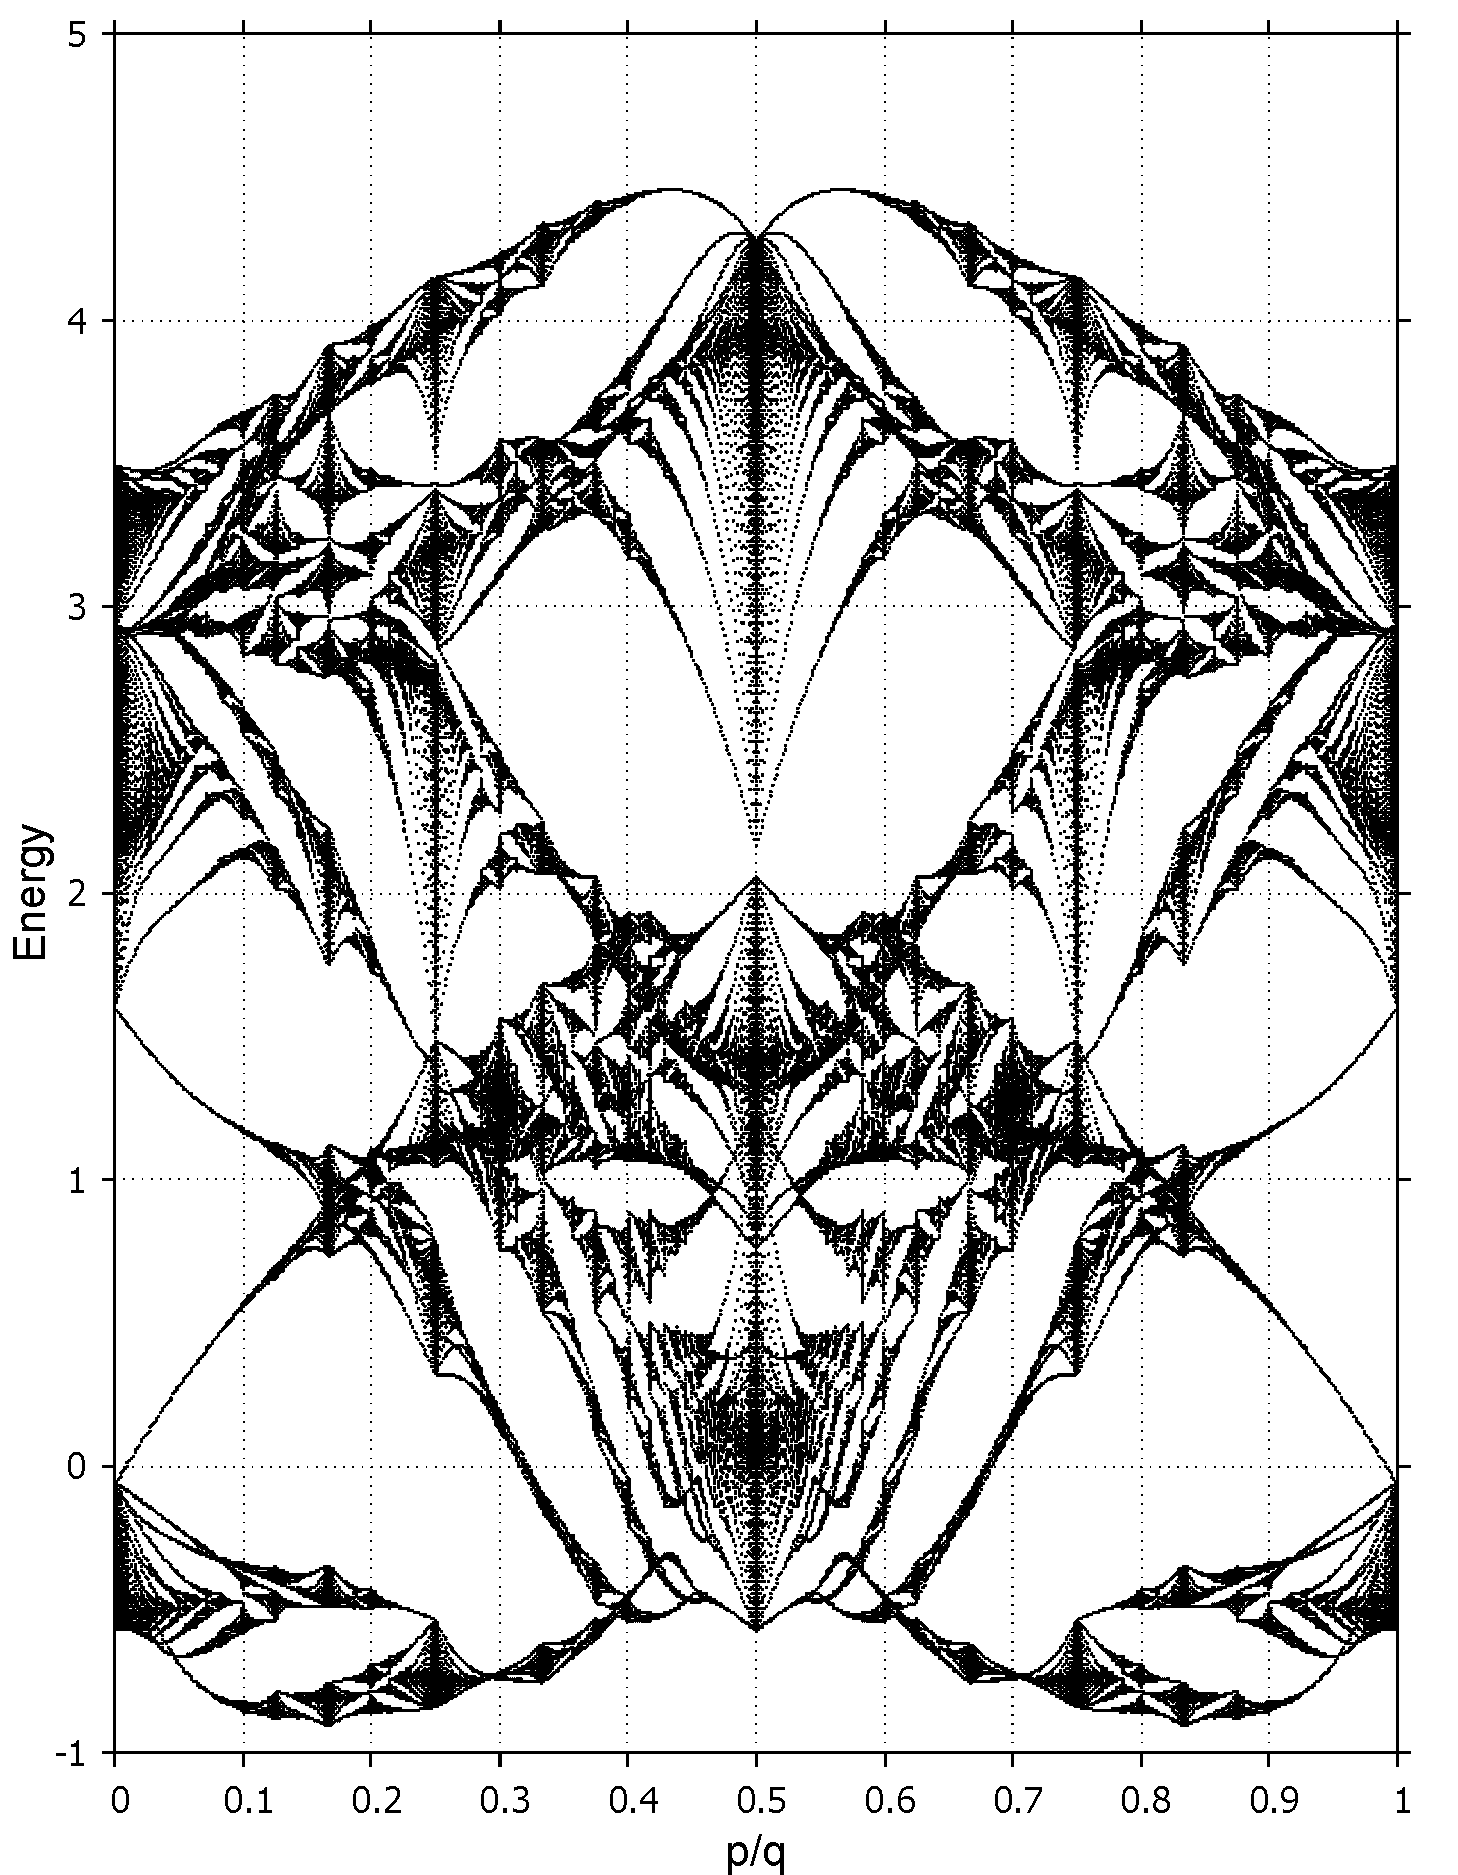
\includegraphics[width=0.7\linewidth]{../pic/3band_gnuplot_q_797.png}
				\end{figure}
				\smallskip
			\end{minipage}
		\end{multicols}
	\end{frame}
	\begin{frame}{Hofstadter butterfly in $MX_{2}$}
		\begin{figure}
			\begin{subfigure}[b]{0.3\linewidth}
				\centering
				\includegraphics[width=0.6\linewidth]{./pic/plotHofstadterButterfly_q=797_MoS2.png}
			\end{subfigure}
			\begin{subfigure}[b]{0.3\linewidth}
				\centering
				\includegraphics[width=0.6\linewidth]{./pic/plotHofstadterButterfly_q=797_MoSe2.png}
			\end{subfigure}
			\begin{subfigure}[b]{0.3\linewidth}
				\centering
				\includegraphics[width=0.6\linewidth]{./pic/plotHofstadterButterfly_q=797_MoTe2.png}
			\end{subfigure}
			\begin{subfigure}[b]{0.3\linewidth}
				\centering
				\includegraphics[width=0.6\linewidth]{../pic/plotHofstadterButterfly_q=797_WS2.png}
			\end{subfigure}
			\begin{subfigure}[b]{0.3\linewidth}
				\centering
				\includegraphics[width=0.6\linewidth]{../pic/plotHofstadterButterfly_q=797_WSe2.png}
			\end{subfigure}
			\begin{subfigure}[b]{0.3\linewidth}
				\centering
				\includegraphics[width=0.6\linewidth]{../pic/plotHofstadterButterfly_q=797_WTe2.png}
			\end{subfigure}
		\end{figure}
	\end{frame}
	\subsection{Landau levels}
	\begin{frame}{Landau levels}
		\begin{figure}
			\centering
			\begin{subfigure}[b]{0.49\textwidth}
				\centering
				{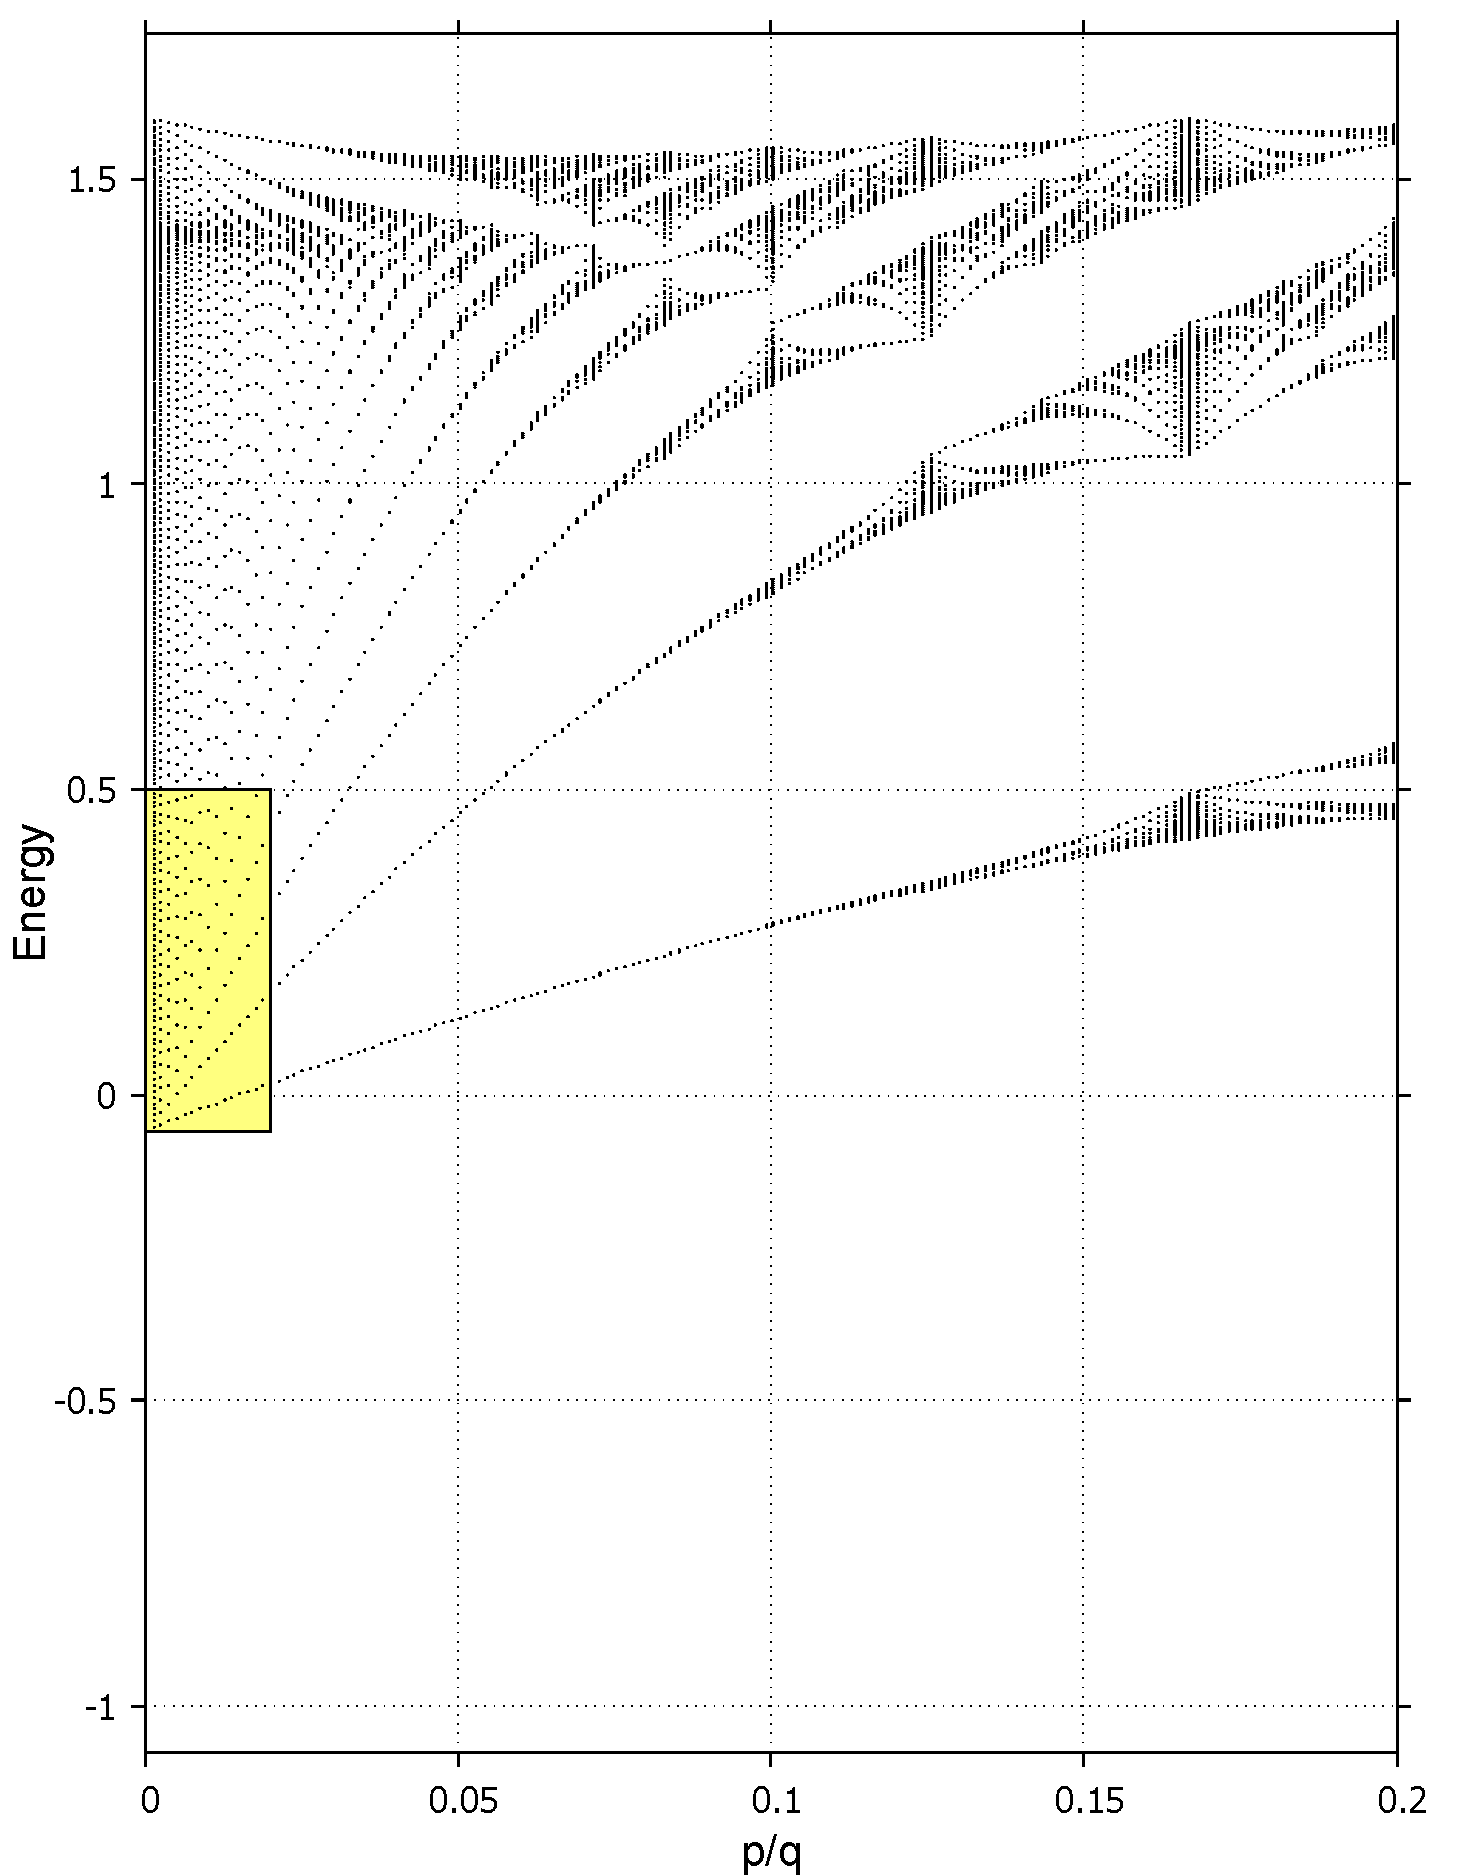
\includegraphics[width=0.6\linewidth]{../pic/small_area_LL.png}}
			\end{subfigure}
			\begin{subfigure}[b]{0.49\textwidth}
				\centering
				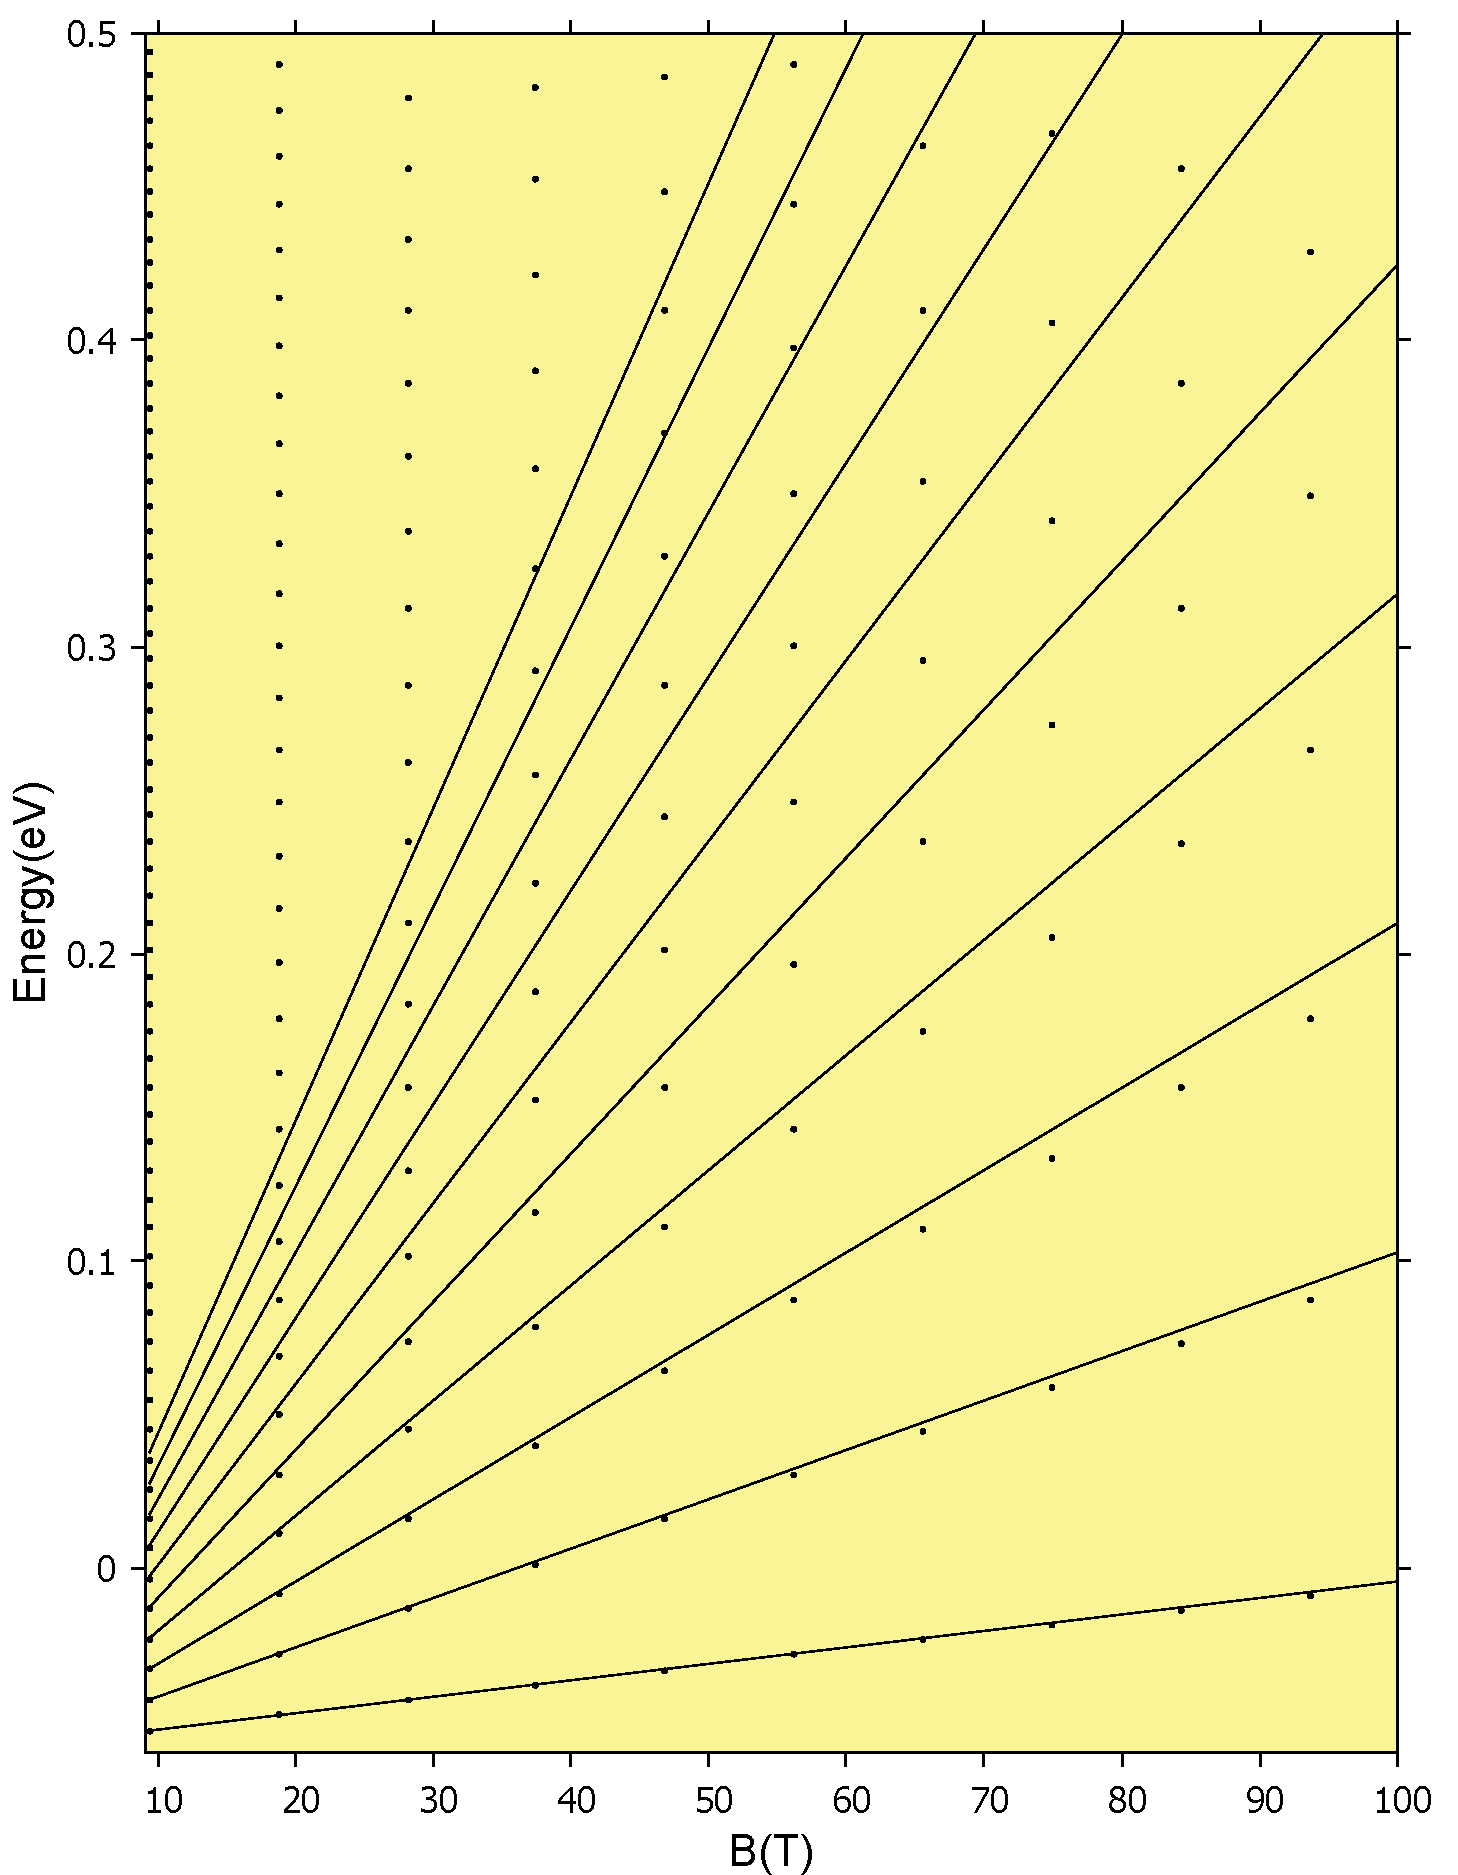
\includegraphics[width=0.6\linewidth]{../pic/landaulevel_h0_q_797.pdf}
			\end{subfigure}
			\caption{
				(a) Same plot as Fig (2.6) but considering a small area and (b) shows superposition of the Landau fan diagram and the Hofstadter butterfly. Display the first $n = 30$ levels near the bottom of the conduction band for a magnetic field up to $B = 500$ T.
			}
		\end{figure}
	\end{frame}
	\subsection{Quantum Hall effect}
	\begin{frame}{Classical Hall effect}
		\note{note text}
	\end{frame}
	\section{Summary and Outlook}
	\begin{frame}
		\begin{block}{Summary:}
			\begin{itemize}
				\item We confirm the Hofstadter butterfly in this model corrected compared to previous study.\\
				\item From three-band TB + magnetic field $\to$ QHE.
			\end{itemize}
		\end{block}
		\begin{exampleblock}{Further research:}
			\begin{itemize}
				\item High Harmonic Generation
				\item High-order Side-band Generation
				\item Photovoltaic effect
			\end{itemize}
		\end{exampleblock}
		\begin{multicols}{2}
			\begin{center}
				\null\vfill
				Thank you for your listening.
				\null\vfill
			\end{center}\columnbreak
		\end{multicols}
		\note[item]{So far, we have used the three-band tight-binding model and semiconductor Bloch equations to calculate the linear absorption spectrum. We confirm that this model matches the results with the experiment data and also predicts smaller exciton peaks.}
		\note[item]{For further results, we can include the many-body interaction in calculating other phenomena for a realistic picture of TMD's properties.}
	\end{frame}
\end{document}